\subsection{SIGMET data format - raw format (Vaisala)}
\label{sigmet}
Vaisala is a Finnish company specializing in environmental and meteorological instrumentation. The RAW format (also referred to as SIGMET in some documents \cite{lrose_RadxConvert}) is one of the storage formats developed by the company to organize data output from their radar devices.

Some notable points about this format include:

\begin{itemize}
    \item The file content is divided into a \textbf{block}, each with a size of exactly 6144 bytes. This size aligns with the main storage size on older tape devices.
    \item The file typically consolidates data from all radar scanning sessions.
    \item Data records are organized within the scope of one block (6144 bytes). In the case of any remaining space in the block, it is padded with additional zeros.
\end{itemize}

With the aforementioned characteristics, the key advantages of the RAW format storage can be identified: \cite{raw_product_format_vaisala}

\begin{itemize}
    \item Compatibility with various tape types, which were commonly used devices in the past and are still widely used due to their cost-effective storage capacity.
    \item Through the use of the block mechanism, SIGMET facilitates block-level error recovery in storage systems.
\end{itemize}

The main concern raised by the team is the mapping capability between the storage structure on the hard drive and on the tape.

\subsection{NETCDF data format - Network Common Data Form}

NetCDF (Network Common Data Form) is a versatile file format designed explicitly for storing multidimensional scientific data. Within the netCDF library system, various binary formats are supported, each contributing to the flexibility and scalability of data management \cite{netcdf}. Notably, these formats include:

\begin{enumerate}
    \item Classic Format: Initially used in the first version of netCDF and remains the default choice for file creation.
    \item 64-bit Offset Format: Introduced since version 3.6.0, this format supports larger variable and file sizes.
    \item netCDF-4/HDF5 Format: Introduced in version 4.0, utilizing the HDF5 data format with some limitations.
    \item HDF4 SD Format: Primarily supports data reading.
    \item CDF5 Format: Synchronized support with the parallel-NetCDF project.
\end{enumerate}

All these formats exhibit self-description, with a detailed header part describing the file structure, including data arrays and file metadata in the form of attribute name/value pairs. This design ensures platform independence, with issues such as endianness being flexibly addressed through software libraries.

Consider a specific example of storing essential meteorological parameters such as temperature, humidity, pressure, wind speed, and direction in netCDF files. This illustrates the capability of this format in handling diverse scientific datasets, providing a powerful and flexible means to manage multidimensional information.

\begin{figure}[H]
    \centering
    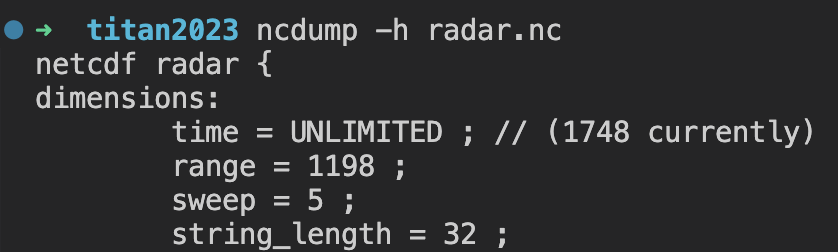
\includegraphics[width=1\linewidth]{Images/ncdump.png}
    \vspace{1em}
    \caption{Radar information in NETCDF format. The total dimensions of the dataset are 2975, grouped into 4 distinct labels.}
    \label{fig:enter-label}
\end{figure}

Starting from version 4.0, the netCDF API introduces the ability to use the HDF5 data format.
This crucial integration allows netCDF users to create HDF5 files, unlocking benefits such as significantly larger file sizes and support for unlimited dimensions.
This step marks a significant move towards leveraging the extended advantages of the HDF5 format.

NetCDF Classic and 64-bit Offset Formats are international standards of the Open Geospatial Consortium \cite{ogcnetcdf}, demonstrating the robustness and reliability in ensuring the compatibility and global scalability of the netCDF format.
